\documentclass[eng,openany]{mgr}
\usepackage{listings}
\usepackage[english]{babel}
\usepackage{graphicx}
\usepackage{hyperref}
\usepackage{tabularx,colortbl} 
\usepackage{rotating}
\usepackage[utf8]{inputenc} 
\setlength\parindent{24pt}
\usepackage[parfill]{parskip}
\usepackage[table,kernelfbox,hyperref]{xcolor}
\usepackage{fancyhdr}
\usepackage{gauss}
%\usepackage[colorinlistoftodos]{todonotes}

\hypersetup{colorlinks=true}
\hypersetup{xurlbordercolor=red!70!black}
\hypersetup{xlinkbordercolor=blue!70!black}
\hypersetup{linkcolor=blue!60!black}
\hypersetup{urlcolor=red!50!black}
\hypersetup{citecolor=green!30!black}
\rfoot{Page \thepage}
\renewcommand\lstlistlistingname{List of Listings}
\newcommand{\linia}{\rule{\linewidth}{0.4mm}}

\definecolor{listlightgray}{gray}{0.97}

\newcommand{\lstsetmylst} {
\lstset{frame = tb,
breaklines=true,
framerule = 0.25pt,
float,
fontadjust,
backgroundcolor={\color{listlightgray}},
basicstyle = {\ttfamily\footnotesize},
identifierstyle = {\ttfamily},
stringstyle = {\ttfamily},
showstringspaces = false,
showtabs = false,
numbers = left,
numbersep = 6pt,
tabsize = 4,
language=C,
floatplacement=!h
}
}

\newcommand{\lstsetatc} {
\lstset{frame = tb,
breaklines=true,
framerule = 0.25pt,
float,
fontadjust,
backgroundcolor={\color{listlightgray}},
basicstyle = {\ttfamily\footnotesize},
keywordstyle = {\ttfamily\color{listkeyword}\textbf},
identifierstyle = {\ttfamily},
commentstyle = {\ttfamily\color{listcomment}\textit},
stringstyle = {\ttfamily},
showstringspaces = false,
showtabs = false,
numbers = left,
numbersep = 6pt,
numberstyle={\ttfamily\color{listnumbers}},
tabsize = 4,
language=C,
floatplacement=!h
}
}

\newcommand{\lstsetatbashnum} {
\lstset{frame = tb,
breaklines=true,
framerule = 0.25pt,
aboveskip=2ex,
float,
fontadjust,
backgroundcolor={\color{listlightgray}},
basicstyle = {\ttfamily\footnotesize},
keywordstyle = {\ttfamily\color{listkeyword}\textbf},
identifierstyle = {\ttfamily},
commentstyle = {\ttfamily\color{listcomment}\textit},
stringstyle = {\ttfamily},
showstringspaces = false,
showtabs = false,
numbers = left,
numbersep = 6pt,
numberstyle={\ttfamily\color{listnumbers}},
tabsize = 4,
language=bash,
floatplacement=!h
}
}
\lstsetmylst
\author{Jaroslaw M. Szumega}
\title{}
\engtitle{}
\supervisor{Rafal Zdunek, D.Sc, K-4/W4}
\field{Electronics}
\specialisation{Advanced Applied Electronics}
\date{21.03.2017}
\begin{document}
\selectlanguage{english}
\maketitle
\tableofcontents
\chapter{Solution to the given problems}
The solutions below are the requested numerical results of requested problems as well as the execution time's comparison between different algorithms. To ensure proper timings, all measurements are made for one thousands rounds/repetition -- it will help to reduce the impact of setting up the Octave engine and other overheads.
\begin{figure}[h]
	\centering
	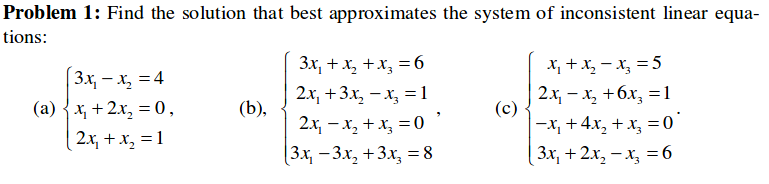
\includegraphics[width=0.6\linewidth]{screenshot001}
	\label{fig:screenshot001}
\end{figure}
\\Each system was solved using set of algorithms dedicated for solving Least Squares problem: there was LS approximation, solving LS using Singular Vector Decomposition (SVD) or QR factorization. In addition the first system is solved also by linear regression.
\begin{lstlisting}
Matrix A
Classical LS
	time =  0.12578
SVD LS
	time =  0.78760
QR LS
	time =  0.061208
regression
	time =  0.087359

Matrix B
Classical LS
	time =  0.043440
SVD LS
	time =  0.86493
QR LS
	time =  0.059717

Matrix C
Classical LS
	time =  0.041433
SVD LS
	time =  0.81831
QR LS
	time =  0.057312
\end{lstlisting}
\begin{figure}[h]
\centering
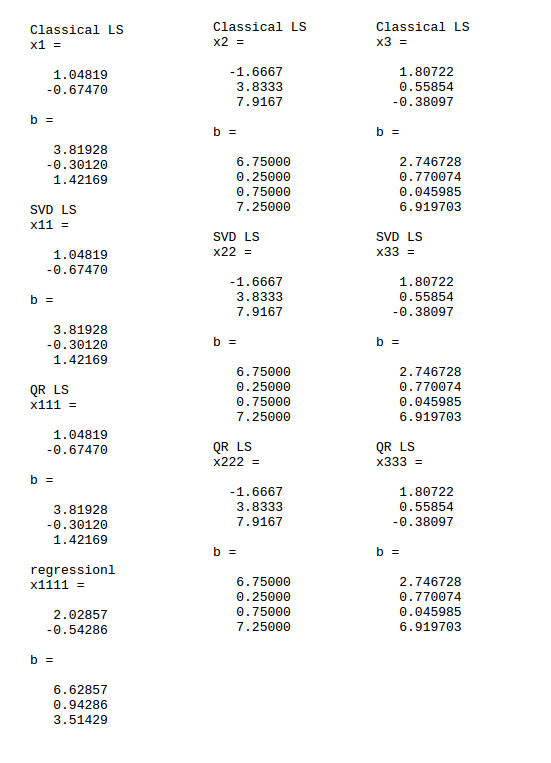
\includegraphics[width=0.7\linewidth]{screenshot003}
\caption{Calculations results. Also verification in form b = Ax}
\label{fig:screenshot003}
\end{figure}
\hspace{40pt}
\newpage
\begin{figure}[h]
\centering
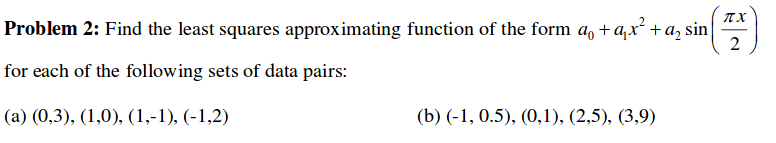
\includegraphics[width=0.7\linewidth]{screenshot004}
\label{fig:screenshot004}
\end{figure}

The selected systems was written in the form of matrices. In Octave code it is like this:
\begin{lstlisting}
A1= [1 0 sin(3.14*0/2);
1 1 sin(3.14*1/2);
1 1 sin(3.14*1/2);
1 1 sin(3.14*(-1)/2); ]

b1 = [3; 0; -1; 2]


# b)
A2 = [1 1 sin(3.14*(-1)/2);
1 0 sin(3.14*0/2);
1 4 sin(3.14*2/2);
1 9 sin(3.14*3/2); ]

b2 = [0.5; 1; 5; 9]
\end{lstlisting}
Then the algorithms were applied to get the solution.

\begin{figure}[h]
	\centering
	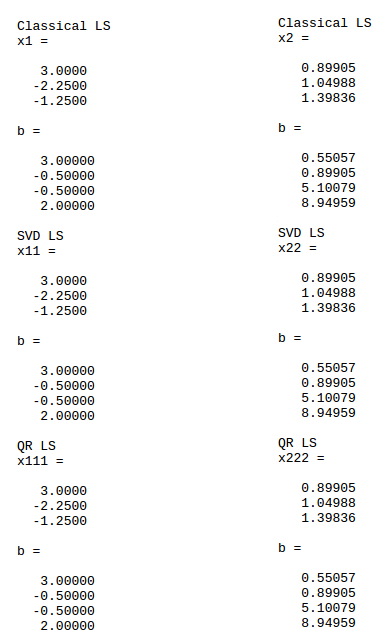
\includegraphics[width=0.5\linewidth]{screenshot005}
	\label{fig:screenshot005}
\end{figure}

As the picture shows, the calculated coefficients gives quite a good approximation, when using them in computing the "b" vector.

The listing below show also timings of selected algorithms:

\begin{lstlisting}

Case A:

Classical LS
	time =  0.050778
SVD LS
	time =  0.73374
QR LS
	time =  0.051985


Case B:

Classical LS
	time =  0.034670
SVD LS
	time =  0.71804
QR LS
	time =  0.051468
\end{lstlisting}
\newpage
\begin{figure}[h]
\centering
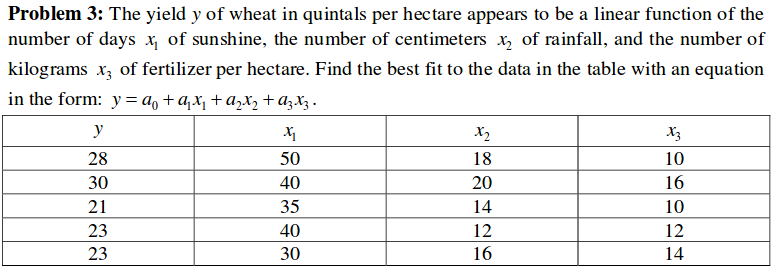
\includegraphics[width=0.7\linewidth]{screenshot006}
\label{fig:screenshot006}
\end{figure}

The problem mentioned above should be presented in form of matrix:
\begin{figure}[h]
\centering
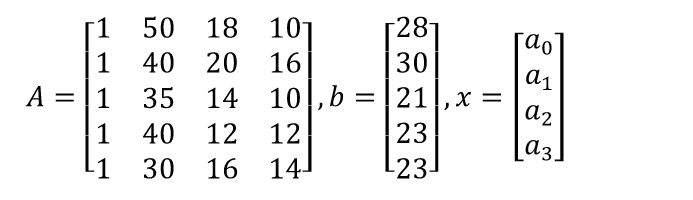
\includegraphics[width=0.5\linewidth]{screenshot007}
\label{fig:screenshot007}
\end{figure}
Once again, the set of selected algorithms will be used. This time there also will be selected the Thikonov regularization.

\begin{figure}[h]
\centering
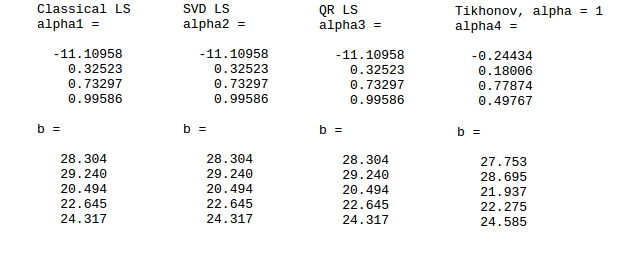
\includegraphics[width=0.7\linewidth]{screenshot008}
\caption{Results.}
\label{fig:screenshot008}
\end{figure}
Looking at \ref{fig:screenshot008} we can see, that all the solutions during the verification give quite good approximation of "b". The first three has exactly the same values and are much better than last algorithm. However, Tikhonov regularization gives the coefficients that stand out of the rest of solutions, but this solution is still correct.

And the timing comparison:
\begin{lstlisting}
Classical LS
time =  0.064596


SVD LS
time =  0.75261


QR LS
time =  0.052665


Gen. Tikhonov, alpha = 1
time =  0.041787
\end{lstlisting}
\newpage
\begin{figure}[h]
\centering
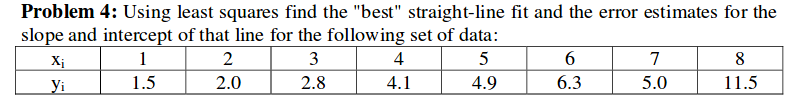
\includegraphics[width=0.7\linewidth]{screenshot009}
\label{fig:screenshot009}
\end{figure}
At first, the problem presented in matrices:
\begin{figure}[h]
\centering
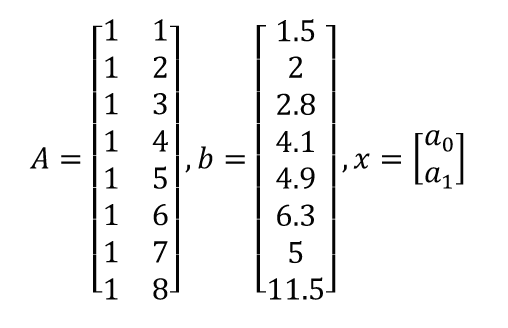
\includegraphics[width=0.35\linewidth]{screenshot010}
\label{fig:screenshot010}
\end{figure}
The results below show the solution computed by different methods. The first three methods are pretty the same answers.
\begin{figure}[h]
\centering
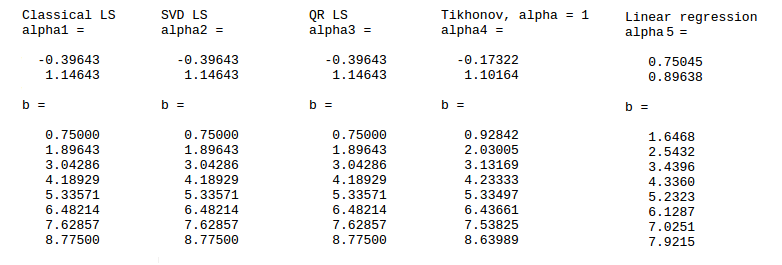
\includegraphics[width=0.8\linewidth]{screenshot011}
\label{fig:screenshot011}
\end{figure}


There were also calculated the timings and the errors of the selected methods:
\begin{lstlisting}
Classical LS
	error =  3.8985
	time =  0.043488
	
SVD LS
	error =  3.8985
	time =  0.72264
	
QR LS
	error =  3.8985
	time =  0.054575
	
Tikhonov, alpha = 1
	error =  3.9098
	time =  0.057088
	
Linear regression
	error =  4.9385
	time =  0.071316
\end{lstlisting}
As it turned out, the best algorithm considering both time and error is the classical LS fitting. The SVD and QR based algorithms gave the same solution, but were slower (especially SVD, which also in previous tasks was slow).
\newpage

\begin{figure}[h]
\centering
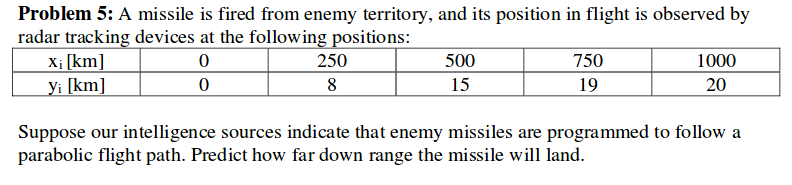
\includegraphics[width=0.7\linewidth]{screenshot012}
\label{fig:screenshot012}
\end{figure}


\chapter{Algorithms code}
Algorithm \space 1 -- The classical LS fitting.\\
\begin{lstlisting}
function [x] = classicLS(A, b)

[m,n] = size(A)

if(m >= n || rank(A) == n)
	disp(["There is an unique solution"])
	x = inv(A' * A) * A' * b;
else if ( m < n)
	disp(["Underdetermined system"])
	x = A' * inv(A * A') * b;
end
endfunction
\end{lstlisting}

Algorithm \space 2 -- Pseudoinverse\\
\begin{lstlisting}
function [x] = pseudoinverse(A)

[m,n] = size(A);
r = rank(A);
[u,s,v] = svdqr(A,20);

x = zeros(n,m);

for i = 1:r
	x = x + inv(s(i,i)) *v(:,i)* u(:,i)';
endfor

endfunction
\end{lstlisting}
\newpage
Algorithm \space 3 -- The orthogonal projectors\\
\begin{lstlisting}
function [Pra, Prah, Pna, Pnah] = projectors(A)

[m,n] = size(A)

Pra = A * pseudoinverse(A)
Prah = pseudoinverse(A) * A

Pnah = eye(size(Pra)) - Pra
Pna = eye(size(Prah)) - Prah

endfunction
\end{lstlisting}

Algorithm \space 4 -- The LS solution by SVD\\

\begin{lstlisting}
function [x] = svdLS(A,b)

[u,s,v] = svd(A);

x = (v*pseudoinverse(s) * u') * b;

endfunctiong
\end{lstlisting}
Algorithm \space 5 -- The LS solution by QR factorization\\
\begin{lstlisting}
function [U, S, V] = svdQR(A,iterations)

[n, m]= size(A); # can be rectangular matrix
U=eye(n);   
V=eye(m);

R=A';  

for i = 0:iterations
	[Q,R]=qr(R');   # qr decompositions and updating  
	U=U*Q;         
	[Q,R]=qr(R');
	V=V*Q;
endfor
S=R';               # S is R transposed

endfunction
\end{lstlisting}
\newpage
Algorithm \space 6 -- The linear regression\\
\begin{lstlisting}
function [x] = regression(A, b)

[m,n] = size(A
[p,r] = size(b);

if(n != 2 || r != 1)
	disp(["The matrix does not describe the polynomial of first degree"])

else
	meanY = sum(b)/p
	meanT = sum(A(:,n))/m
	
	#beta = (sum(b.*A(:,n)) - m*meanY*meanT)/(sum(A(:,n).^2) - m * meanT*meanT)
	#alpha = meanY - beta*meanT
	
	#more accurate b calculation
	first = (b.- meanY).*(A(:,n).-meanT)
	second = (b.-meanT).^2
	beta = sum(first)/sum(second)
	alpha = meanY - beta*meanT
	
	x = [alpha;beta]
endif
endfunction
\end{lstlisting}
Algorithm \space 7 -- The TSVD algorithm\\
\begin{lstlisting}
function [x] = tsvd(A,b, it)

[u,s,v] = svdqr(A,it);

c = u'*b
r = rank(A)
x=zeros(size(A,2),1);

for i = 1:r
	x = x + (c(i)*v(:,i))/s(i,i);
endfor
endfunction
\end{lstlisting}
Algorithm \space 8 -- The iterative refinement\\
\begin{lstlisting}
function [x] = refinement(A,x,b,it)

for s = 1:it
	r = b - A*x
	
	#extended refinement
	delta = qrLS(A,r);
	x = x + delta
endfor
endfunction
\end{lstlisting}
Algorithm 10 -- The General Cross-Validation\\
\begin{lstlisting}
function [x] = crossvalidation(A,b, mi)

C = inv(A'*A);
M = A' * A + (mi.^2).^C'*C;

x = inv(M)*A'*b;

endfunction
\end{lstlisting}
Algorithm 11 -- The Iterative Tikhonov Regularization\\
\begin{lstlisting}
function [x] = tikhonovIt(A,b, it, mi)

[m,n] = size(A);

x=zeros(size(A,2),1);
for i = 1:it
	x = x + inv(A' * A + eye(size(A'*A)).*mi) * A' * (b-A*x);
endfor

endfunction
\end{lstlisting}
Algorithm ** -- The General Tikhonov Regularization\\
\begin{lstlisting}
function [x] = tikhonovGen(A,b, alpha)

x = inv(A' * A + alpha.*eye(size(A'*A))) * A' * b;

endfunction
\end{lstlisting}
\newpage
\section{Code for solving particular tasks}
Task1
\begin{lstlisting}
A1 = [3 -1; 1 2; 2 1];
b1 = [4; 0; 1];

disp(["Classical LS"])
tic
for i = 1:1000
x1 = classicLS(A1,b1);
endfor
time = toc

disp(["SVD LS"])
tic
for i = 1:1000
x11 = svdLS(A1,b1);
endfor
time = toc

disp(["QR LS"])
tic
for i = 1:1000
x111 = qrLS(A1,b1);
endfor
time = toc

disp(["regressionl"])
tic
for i = 1:1000
x1111 = regression(A1,b1);
endfor
time = toc

[...]

The similar calculations are performed for the remaining matrices.
\end{lstlisting}
\begin{thebibliography}{8}
\addcontentsline{toc}{chapter}{Bibliography}
%\addcontentsline{toc}{section}{Literatura}
\bibitem{bjorck}
Björck, Åke. Numerical methods for least squares problems. Society for Industrial and Applied Mathematics, 1996.
\bibitem{golub}
Golub, Gene H., and Charles F. Van Loan. "Matrix computations, 3rd." (1996).
\bibitem{zdunek}
Zdunek R., Numerical Methods - lecture slides.
\end{thebibliography}

\end{document}

